% !TeX spellcheck = en_GB
% !TeX encoding = UTF-8
% IMEKO World Congress 2027 (Rimini) -- Extended Abstract, track TC21.
% Official class imeko_wc v2.5. Build:
%   pdflatex extended_abstract && bibtex extended_abstract
%   pdflatex extended_abstract && pdflatex extended_abstract
% Every number in this file is traced to its source in NUMBERS.md and is
% recomputed by check_numbers.py.

\documentclass{imeko_wc}
\usepackage[british]{babel}
\DeclareSIUnit\year{yr}

\graphicspath{{../../figures/}{figures/}}

\begin{document}

\title{Surrogates for Monte Carlo uncertainty propagation with twenty model
runs}

\author[a1]{name=Yugam Jinesh, surname=Vora, abbreviation=Y. J. Vora}
\author[a2]{name=Wee Hoe, surname=Ng, abbreviation=W. H. Ng}
\affiliation[a1]{Department of Engineering Science, National University of
Singapore, Singapore}
\affiliation[a2]{National Metrology Centre, Agency for Science, Technology and
Research (A*STAR), Singapore}
\CorrespondingAuthorNumber{1}
\CorrespondingAuthorEmail{yugam@u.nus.edu}
\funding{}

\maketitle

\begin{abstract}
Monte Carlo propagation of distributions needs far more model evaluations
than an expensive simulation allows, so the model is replaced by a surrogate trained on about twenty runs. We compare surrogate
strategies on four test models, including a Gaussian plume model of an
ammonia release, over 30 paired repetitions, scoring propagated quantiles
and exceedance probabilities against reference Monte Carlo values. The
kernel specification of a Gaussian process changed the error up to
eighteen-fold; one hyperparameter held fixed produced an apparent failure
that an earlier analysis attributed to domain size. Logarithmic
transformation of positive variables reduced the error up to eightfold.
Committees of surrogates beat a well-specified Gaussian process
only where one member matched the response structure, and only with error
weighting; the adaptive designs tested gave no consistent gain.
Cross-validation estimated the surrogate error conservatively; the Gaussian
process's own predictive uncertainty understated it up to threefold.
\end{abstract}

\begin{keywords}
Measurement uncertainty; Monte Carlo method; Surrogate model; Gaussian process;
Computer experiments
\end{keywords}

\section{Introduction}
Evaluating measurement uncertainty by the propagation of distributions,
following Supplement~1 to the Guide to the Expression of Uncertainty in
Measurement (GUM~S1)~\cite{jcgm100,jcgm101}, requires the measurement model
$Y=f(\mathbf{X})$ to be evaluated once per Monte Carlo trial, typically
$10^5$ to $10^6$ times~\cite{cox2006,harris2014}. For many quantities of
practical interest, $f$ is itself a numerical simulation. One example is the
concentration downstream of an accidental ammonia release~\cite{tan2017}: a
single computational fluid dynamics (CFD) run takes hours to days, and a
practical budget is often fewer than twenty runs.

The usual remedy is a \emph{surrogate} (emulator) trained on those runs and
used in place of $f$ inside the Monte Carlo loop~\cite{heidenreich2017,
wang2022,ohagan2006}. The surrogate's error then becomes a contribution to the
uncertainty budget~\cite{kennedy2001}. Gaussian process (GP)
regression~\cite{sacks1989,rw2006} is the standard surrogate; a common
guideline asks for about ten runs per input~\cite{loeppky2009}, which many
applications cannot afford, and results are known to depend on modelling
choices~\cite{chen2016}. Several alternatives have been proposed for small
budgets: weighted committees of different surrogates~\cite{goel2007,
viana2009}, adaptive selection of runs~\cite{gramacy2009} and, recently,
spectral measures of disagreement~\cite{lin2024}.

An earlier analysis of such a scheme (heterogeneous committee, spectral
acquisition, dynamic model management) reported that a passively sampled GP
fails catastrophically on large input domains and that the committee recovers
accuracy. This contribution tests which of those conclusions survive a
controlled comparison with correctly specified baselines, scores the
strategies on the quantities a GUM~S1 evaluation reports, and asks how far the
surrogate's own error can be estimated from the training runs alone.

\section{Proposed contribution}
\subsection{Test models}
Four models with uniform input distributions are used (Table~\ref{tab:models}).
\emph{Physics} is the benchmark of the earlier analysis; its dominant
quadratic term lies exactly in the class of one committee member.
\emph{Plume} is the ground-level concentration of a continuous ammonia
release from a Gaussian plume model with Briggs rural dispersion coefficients
for neutral stability and ground reflection. Its output spans three orders of
magnitude and has a \qty{12}{\percent} probability of exceeding the level
immediately dangerous to life or health (IDLH) for ammonia,
\qty{210}{\milli\gram\per\cubic\metre} (about \num{300} ppm). The plume model
is an analytical, controlled proxy for dispersion problems, cheap enough for
exact reference values; it is not a CFD simulation, and CFD responses with
recirculation or regime changes may behave differently. \emph{Borehole}
(water flow) and \emph{Ishigami} are standard test functions for computer
experiments. No committee member matches the last three.

\begin{table}[tb]
\centering
\caption{Test models; $d$: number of inputs.}
\label{tab:models}
\begin{tabular}{lrl}
\toprule
Model & $d$ & Inputs; output\\
\midrule
Physics  & 3 & $[-200,200]^3$\\
Plume    & 5 & release, wind, height, distance, offset;\\
         &   & concentration in \si{\milli\gram\per\cubic\metre}\\
Borehole & 8 & standard ranges; flow in \si{\cubic\metre\per\year}\\
Ishigami & 3 & $[-\uppi,\uppi]^3$\\
\bottomrule
\end{tabular}
\end{table}

\subsection{Strategies}
Every strategy uses $N=20$ runs of the model. The single-GP strategies use a
20-point Latin hypercube with five kernel specifications: the original kernel
of the earlier analysis, a squared exponential with one length scale whose
amplitude is \emph{fixed} at 1 on the standardised output (not estimated);
with the amplitude estimated; with one length scale per input (automatic
relevance determination, ARD); with both; and a Mat\'ern-5/2 ARD kernel with
amplitude. Hyperparameters are estimated by maximising the log marginal
likelihood (L-BFGS-B, five random restarts) on standardised inputs and
outputs, with length scales in $[10^{-2},10^{3}]$, amplitude in
$[10^{-3},10^{3}]$ and a nugget variance in $[10^{-8},10^{-1}]$. A further
variant fits the Mat\'ern GP to the logarithm of the output, with logarithmic
transformation of inputs whose range is strictly positive (plume and borehole
only); its predictions are back-transformed as the exponential of the latent
mean, i.e.\ the predictive median, without bias correction. The adaptive GP
starts from five Latin hypercube runs and adds 15 at its largest posterior
standard deviation~\cite{gramacy2009}.

The committee has nine members: two GPs (with amplitude and ARD), polynomial
chaos expansions (PCE)~\cite{xiu2002,sudret2008} of degrees 2 and 3, two
random forests, a support vector regressor and two neural networks. Its
members are combined either uniformly or with weights
\begin{equation}
w_k\propto\left[\mathrm{MSE}_{\mathrm{CV},k}\,(1+\pi_k)\right]^{-1},
\label{eq:w}
\end{equation}
where $\mathrm{MSE}_{\mathrm{CV},k}$ is the three-fold cross-validation error
of member $k$ and $\pi_k\ge0$ penalises predictions below a known physical
bound~\cite{goel2007,viana2009}. The committee is trained either on the
20-point design (passive) or on five runs plus 15 chosen where its weighted
members disagree most (adaptive). Disagreement is scored by the variance of
the member predictions or by UEigV, the eigenvalue-based measure that Lin et
al.~\cite{lin2024} derived from the normalised graph Laplacian of pairwise
similarities between sampled language-model outputs; here the graph is built
from the $K$ member predictions at a candidate input.

\subsection{Evaluation}
Each strategy is run with 30 seeds. Seeds are shared, so passive strategies
use the identical design and adaptive strategies the identical start. The
trained surrogate propagates \num{3e4} input draws, and the propagated mean,
standard deviation (SD) and 95th percentile $y_{0.95}$ are compared with a
reference Monte Carlo evaluation of the true model ($M=\num{2e5}$). Two
exceedance assessments are distinguished: $P(Y>y_{0.95})$ at the reference
95th percentile, whose true value is 0.05 by construction and which tests
tail accuracy on every model; and, for the plume, $P(C>\mathrm{IDLH})$ at a
fixed physical threshold, which is the quantity a risk decision uses.
Accuracy over the input domain is the root mean square error (RMSE) on 5000
test points divided by the output SD (normalised RMSE; 1 corresponds to a
constant predictor). Strategies are compared by two-sided Wilcoxon
signed-rank tests on paired $\log$ normalised RMSE; the 36 tests reported are
treated as exploratory, and $p$-values are Holm-adjusted for multiplicity.
All of these errors are \emph{validation} errors that need the reference
model; Section~\ref{sec:estimate} examines what can be estimated without it.
Code and every per-seed record are openly available~\cite{repo}.

\section{Preliminary results and potential applications}
\subsection{Kernel specification and variable transformation}
Table~\ref{tab:kernel} shows that the specification of a single GP matters
more than any other choice examined. On the physics model the original kernel
reaches 0.59, close to a constant predictor; estimating the amplitude alone
reduces this to 0.033 (all 30 seeds improve, adjusted $p<10^{-6}$). The
catastrophic GP failure reported earlier is therefore a specification
artefact (Fig.~\ref{fig:dom}): with the amplitude fixed, the normalised RMSE
is 0.60 at every domain half-width from 10 to 200, whereas a Mat\'ern-5/2 ARD
GP with amplitude reaches 0.17 at 10 and 0.08 from 50 to 200. The committee
remains far more accurate on this model, but because of its degree-2 PCE
member, not because the GP fails. On the borehole model ARD matters (0.30 to
0.09). Logarithmic transformation then gives the largest single improvement:
from 0.089 to 0.011 on the borehole model and from 0.60 to 0.42 on the plume
(30 and 27 of 30 seeds improve; adjusted $p<10^{-6}$ and $p<10^{-3}$). No GP
does better than 0.9 on the Ishigami function, for which the
ten-runs-per-input guideline~\cite{loeppky2009} would ask for 30 runs.

\begin{figure}[tb]
\centering
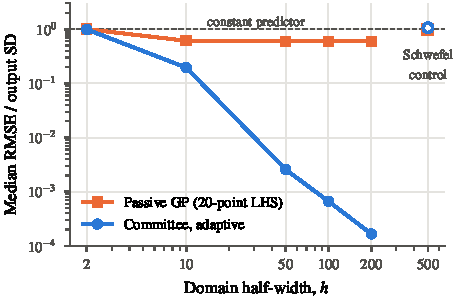
\includegraphics[width=\columnwidth]{fig_domain_sweep}
\caption{Physics model on $[-h,h]^3$: median normalised RMSE over 30 seeds
against the domain half-width. Open markers: Schwefel function on
$[-500,500]^3$. Dashed line: constant predictor.}
\label{fig:dom}
\end{figure}

\begin{table}[tb]
\centering
\caption{Median normalised RMSE of a single GP on a 20-point Latin hypercube,
30 seeds. Amp.: amplitude estimated; Mat\'ern: Mat\'ern-5/2 kernel.}
\label{tab:kernel}
\begin{tabular}{lrrrr}
\toprule
Kernel & Phys. & Plume & Boreh. & Ishig.\\
\midrule
Original (amp. fixed)    & 0.591 & 0.602 & 0.295 & 0.956\\
+ amp.                   & 0.033 & 0.590 & 0.247 & 0.970\\
+ ARD                    & 0.608 & 0.632 & 0.129 & 1.01\\
+ amp. + ARD             & 0.036 & 0.596 & 0.085 & 0.896\\
Mat\'ern, amp. + ARD     & 0.079 & 0.597 & 0.089 & 0.902\\
\quad on log variables   & --    & 0.418 & 0.011 & --\\
\bottomrule
\end{tabular}
\end{table}

\begin{figure}[tb]
\centering
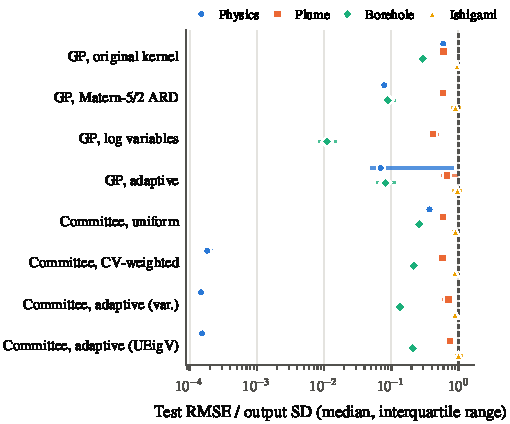
\includegraphics[width=\columnwidth]{fig_strategies}
\caption{Normalised RMSE of each strategy on each test model: median (marker)
and interquartile range (bar) over 30 seeds; logarithmic axis. Dashed line:
constant predictor. Committees use GP members with amplitude and ARD.}
\label{fig:strategies}
\end{figure}

\subsection{Committees and adaptive runs}
Fig.~\ref{fig:strategies} compares all strategies. A committee outperforms
the best single GP only on the physics model, by more than two orders of
magnitude, and only because the degree-2 PCE represents its dominant term
exactly; the weights then concentrate on that member. On the borehole model
the CV-weighted committee is 2.3 times worse than the Mat\'ern-5/2 GP on the
same design (0 of 30 seeds better), and on the plume and Ishigami models the
two tie. Uniform averaging was worse than CV weighting on the physics (by a
factor of about 2000) and borehole models (adjusted $p\le0.002$) and never
better. Within the designs tested (five initial runs, 15 adaptive runs chosen
by posterior SD, committee variance or UEigV), adaptive selection gave no
consistent benefit. For the single GP it was never significantly better. For
the committee it helped on the physics and borehole models (median ratios
0.80 and 0.61), hurt on the plume (1.25, adjusted $p=0.005$) and made no
difference on the Ishigami function. UEigV was never better than variance
acquisition after adjustment, and worse on the borehole model by a factor of
1.7 (adjusted $p<10^{-6}$). Acquisition functions aimed at a specific
quantile or threshold may behave differently.

\begin{table*}[tb]
\centering
\caption{Propagation validation error against the reference Monte Carlo
evaluation, median over 30 seeds: relative error (\%) of the mean and of
$y_{0.95}$, and absolute error ($\times100$) of $P(Y>y_{0.95})=0.05$. Bold:
best per column.}
\label{tab:prop}
\begin{tabular}{l rrr rrr rrr rrr}
\toprule
& \multicolumn{3}{c}{Physics} & \multicolumn{3}{c}{Plume} &
\multicolumn{3}{c}{Borehole} & \multicolumn{3}{c}{Ishigami}\\
\cmidrule(lr){2-4}\cmidrule(lr){5-7}\cmidrule(lr){8-10}\cmidrule(lr){11-13}
Strategy & mean & $y_{0.95}$ & $P$ & mean & $y_{0.95}$ & $P$ &
mean & $y_{0.95}$ & $P$ & mean & $y_{0.95}$ & $P$\\
\midrule
GP, original kernel & 8.90 & 21.1 & 4.86 & 10.4 & 20.4 & 3.29 & 1.60 & 13.0 & 4.25 & 10.3 & 34.6 & 4.73 \\
GP, Mat\'ern-5/2 ARD & 1.36 & 3.88 & 1.37 & 9.68 & 17.7 & 2.87 & 0.66 & 2.45 & 0.91 & \textbf{8.48} & \textbf{16.0} & 3.61 \\
GP, log variables & -- & -- & -- & \textbf{4.74} & \textbf{6.94} & \textbf{0.76} & \textbf{0.17} & \textbf{0.60} & \textbf{0.18} & -- & -- & -- \\
Committee, CV-weighted & \textbf{0.21} & \textbf{0.41} & \textbf{0.15} & 8.75 & 23.1 & 3.15 & 1.06 & 10.9 & 3.05 & 11.0 & 28.7 & \textbf{2.89} \\
Committee, adaptive & \textbf{0.21} & \textbf{0.41} & \textbf{0.15} & 55.1 & 20.5 & 5.39 & 3.30 & 1.41 & 0.49 & 15.9 & 34.9 & 4.40 \\
\bottomrule
\end{tabular}
\end{table*}

\subsection{Propagated quantities}
Table~\ref{tab:prop} gives the validation errors of the quantities a GUM~S1
evaluation reports, and they follow the normalised RMSE. With the best
strategy for each model, the 95th percentile is within \qty{0.41}{\percent}
(physics), \qty{6.9}{\percent} (plume), \qty{0.60}{\percent} (borehole) and
\qty{16}{\percent} (Ishigami) of the reference, and $P(Y>y_{0.95})$ within
0.0015, 0.0076, 0.0018 and 0.029 of 0.05. At the fixed IDLH threshold
(reference $P(C>\mathrm{IDLH})=0.123$), the log-variable GP has a median
absolute error of 0.009 over 30 seeds and the raw-variable GP 0.023;
Fig.~\ref{fig:plume} shows one seed. Adaptive runs can mislead: the adaptive
committee estimated the plume mean with a median error of
\qty{55}{\percent}.

\begin{figure}[tb]
\centering
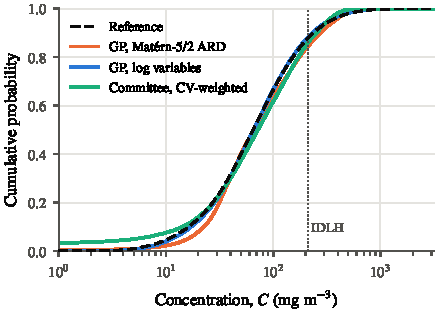
\includegraphics[width=\columnwidth]{fig_plume_cdf}
\caption{Plume model, first seed: distribution of the ground-level
concentration propagated through three surrogates fitted to the same 20 runs,
and the reference Monte Carlo distribution. Dotted: IDLH level for ammonia.}
\label{fig:plume}
\end{figure}

\subsection{Estimating the surrogate contribution}
\label{sec:estimate}
In a real evaluation the reference is unavailable, and the surrogate's
contribution must be estimated from the twenty runs. Table~\ref{tab:est}
compares two estimates with the true error for the recommended GPs: the
five-fold cross-validation RMSE (hyperparameters re-fitted in every fold) and
the root mean square of the GP's own predictive SD. Cross-validation was
conservative: it was at least the true error in 28 and 30 of 30 seeds on the
physics and borehole models, close to it on the plume and Ishigami models,
and below half of it in at most 6 of 30 seeds (plume, log variables). The
GP's own uncertainty was unreliable in the unsafe direction where the GP is
weakest: on the plume and Ishigami models it understated the error by a
factor of 1.7 to 2.8, and its nominal \qty{95}{\percent} predictive intervals
covered 73 to \qty{77}{\percent} of test points. The member envelope of a
committee was no better a substitute: read as an interval for
$P(Y>y_{0.95})$, it contained the reference value in 0 to
\qty{100}{\percent} of seeds depending on model and strategy~\cite{ferson1996}.

\begin{table}[tb]
\centering
\caption{Estimating the surrogate error from the 20 runs, median over 30
seeds: ratio of the five-fold cross-validation RMSE and of the GP's
root-mean-square predictive SD to the true RMSE, and coverage of the nominal
\qty{95}{\percent} predictive interval. M: Mat\'ern GP; L: on log variables.}
\label{tab:est}
\begin{tabular}{llrrr}
\toprule
Model & GP & CV / true & SD / true & Coverage\\
\midrule
Physics  & M & 9.06 & 1.58 & \qty{100}{\percent}\\
Plume    & M & 0.99 & 0.36 & \qty{77}{\percent}\\
Plume    & L & 0.81 & 0.42 & \qty{73}{\percent}\\
Borehole & M & 2.11 & 0.79 & \qty{90}{\percent}\\
Borehole & L & 2.61 & 1.45 & \qty{99}{\percent}\\
Ishigami & M & 1.07 & 0.58 & \qty{73}{\percent}\\
\bottomrule
\end{tabular}
\end{table}

These results suggest a simple, conservative treatment for a GUM~S1
evaluation: propagate $Y=\hat f(\mathbf{X})+E_{\mathrm s}$, where $\hat f$ is
the surrogate and the surrogate error $E_{\mathrm s}$ is an additional input
with expectation zero and standard uncertainty equal to the cross-validation
RMSE. This ignores the spatial variation and correlation of the surrogate
error and inflates the uncertainty when the surrogate is accurate; its
calibration on a CFD case, for example by conformal
prediction~\cite{angelopoulos2023}, is the main task for the final paper.

\subsection{Potential applications}
For surrogate-based GUM~S1 evaluations with about twenty runs, such as a
dispersion study in a risk assessment, the results suggest five rules.
\emph{Specify the GP fully}: estimate an amplitude and one length scale per
input. \emph{Transform the variables} when the model is multiplicative or
positive, for example concentrations and flows. \emph{Use a committee only
with error weighting}, and expect a gain only when a member can represent the
dominant structure. \emph{Prefer a space-filling design} unless an adaptive
criterion has been shown to help for the quantity of interest.
\emph{Estimate the surrogate contribution by cross-validation} and include it
in the budget, rather than relying on the GP's own predictive variance or on
committee spread.

\section{Conclusions}
For Monte Carlo uncertainty propagation with twenty runs of an expensive
model, the kernel specification of a GP surrogate and the transformation of
the variables mattered more than the choice between single surrogates,
committees and the adaptive designs tested. A failure of GP surrogates
reported in an earlier analysis was caused by one hyperparameter held fixed.
Committees helped only when a member matched the response structure and only
with cross-validation error weighting. Cross-validation gave a conservative
estimate of the surrogate's error, whereas the GP's own uncertainty could not
be trusted. These findings rest on analytical models; the final paper will
add a CFD dispersion case, budgets other than twenty runs, and a calibrated
treatment of the surrogate contribution.

\section*{AUTHORS' CONTRIBUTION}
Yugam Jinesh Vora: conceptualisation, methodology, software, investigation,
formal analysis, visualisation, writing -- original draft. Wee Hoe Ng:
conceptualisation, supervision, writing -- review and editing.

\bibliographystyle{imeko_wc}
\bibliography{references}

\end{document}
